
\section{Spray : un protocole d'échantillonnage adaptatif}

\SPRAY est un protocole d'échantillonnage de paris adaptatif inspiré à la fois
de \SCAMP~\cite{ganesh2003peer} et \CYCLON~\cite{voulgaris2005cyclon}. \SPRAY
comprend trois parties représentant le cycle de vie d'un pair dans le
réseau. Tout d'abord, le processus consistant à rejoindre le réseau, qui injecte
un nombre logarithmique d'arcs comparé à la taille du réseau. De ce fait, le
nombre d'arcs passe à l'échelle. Ensuite, chaque pair éxecute un processus
periodique dont le but est d'équilibrer les vues partielles en termes de taille
et d'uniformité sur les pairs références dans celles-ci. Le réseau converge
rapidement vers une topologie possédant des propriétés similaires à celles des
graphes aléatoires. Enfin, un pair est capable de quitter le réseau à n'importe
quel moment sans en notifier le réseau (l'équivalent d'un crash) sans dégrader
les propriétés du reste du réseau.

L'obtention de cette propriété d'adaptivité repose essentiellement sur le fait
de conserver un nombre d'arcs cohérent durant tout le cycle de vie du réseau.
En effet, en opposition à \CYCLON, \SPRAY est toujours à la limite du nombre
optimal d'arcs. Comme \SPRAY n'ajoute jamais d'arcs après le processus d'entrée,
toute suppression d'arcs est définitive et ne doit donc pas être pris à la
légère. Ainsi, \SPRAY ajoute des arcs dans un premier temps. Dans un second
temps, le processus periodique de mélange des arcs de \SPRAY préserve tous les
arcs du réseau.  Dans un troisième temps, le processus de sortie supprime
précautionneusement quelques arcs. Dans l'idéal, il s'agit du nombre d'arcs
ajouté par le dernier pair entré dans le réseau.

Parfois, conserver le nombre d'arcs global constant force les processus de
mélange et de sortie à créer des doublons dans les vues partielles. Ainsi, une
vue partielle peut contenir plusieurs fois le même voisin. Toutefois, ces
doublons restent peu nombreux, et de ce fait, n'ont pas d'impact notable sur la
connectivité du réseau.

\subsection{Rejoindre le réseau}

L'algorithme pour rejoindre le réseau est, dans \SPRAY, la seule manière
d'introduire de nouveaux arcs dans le réseau. Afin de répondre à la première
partie de l'énoncé du problème (REF), ce nombre d'arcs doit augmenter
logarithmiquement comparé à la taille du réseau. Tout comme dans \SCAMP, nous
supposons que chacuns des pairs respecte cette contrainte. Dès lors, ces
derniers utilisent ce savoir afin de propager l'identité du nouvel
arrivant. L'algorithme~\ref{algo:joining} décrit la façon dont le contact envoie
la nouvelle identité à son voisinage où elle est intégrée directement à leur vue
partielle. En définitive, le nombre d'arcs dans le réseau augmente de
$1+\ln(|\mathcal{N}|)$ et ce, seulement en utilisant des interactions de voisin
à voisin.

\begin{figure*}
  \centering
  \subfloat[Figure A][$p_1$ contacts $p_2$ to join the network. $p_1$ adds
  $p_2$ to its neighborhood. $p_1$ sends its request to $p_2$.]{
    
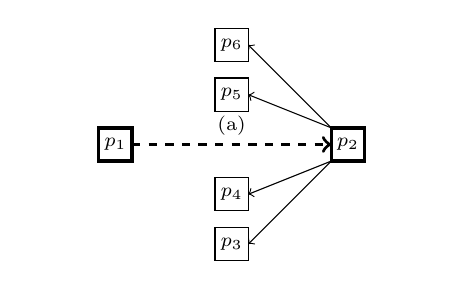
\begin{tikzpicture}[scale=1.2]

  \newcommand\X{35pt};
  \newcommand\Y{15pt};

  \draw(-0.75*\X, 0pt); %% positioning
  \draw( 2.75*\X, 0pt); %% positioning

  \scriptsize
  \draw[->,dashed,very thick](5+0*\X, 0*\Y) -- 
  node[anchor=south]{(a)}(-5+ 2*\X, 0*\Y);
  \draw[->] (-5+2*\X, 5pt) -- (5+\X, \Y);
  \draw[->] (-5+2*\X, 5pt) --  (5+\X, 2*\Y);
  \draw[->] (-5+2*\X, -5pt) -- (5+\X, -\Y);
  \draw[->] (-5+2*\X, -5pt) -- (5+\X, -2*\Y);

  \draw[fill=white, very thick]
  (0*\X, 0*\Y) node{$p_1$} +(-5pt,-5pt) rectangle +(5pt,5pt);
  \draw[fill=white, very thick]
  (2*\X, 0*\Y) node{$p_2$} +(-5pt,-5pt) rectangle +(5pt,5pt);

  \draw[fill=white](1*\X,2*\Y) node{$p_6$} +(-5pt,-5pt) rectangle +(5pt,5pt);
  \draw[fill=white](1*\X,1*\Y) node{$p_5$} +(-5pt,-5pt) rectangle +(5pt,5pt);
  \draw[fill=white](1*\X,-1*\Y) node{$p_4$} +(-5pt,-5pt) rectangle +(5pt,5pt);
  \draw[fill=white](1*\X,-2*\Y) node{$p_3$} +(-5pt,-5pt) rectangle +(5pt,5pt);
  
\end{tikzpicture}}
  \hspace{8pt}
  \subfloat[Figure B][The $onSubs(p_1)$ event is raised at $p_1$
  which forwards the subscription to $p_1$'s neighborhood.]{
    
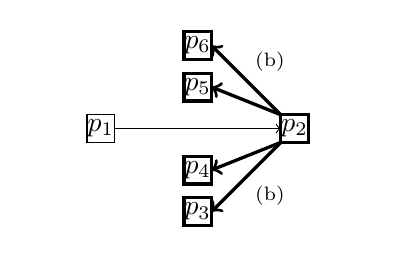
\begin{tikzpicture}[scale=1]

  \newcommand\X{35pt};
  \newcommand\Y{15pt};

  \draw(-0.75*\X, 0pt); %% positioning
  \draw( 2.75*\X, 0pt); %% positioning

  \scriptsize
  \draw[->](5+0*\X, 0*\Y) -- (-5+ 2*\X, 0*\Y);
  \draw[->, very thick] (-5+2*\X, 5pt) -- (5+\X, \Y);
  \draw[->, very thick] (-5+2*\X, 5pt) --
  node[anchor=south west]{(b)} (5+\X, 2*\Y);
  \draw[->, very thick] (-5+2*\X, -5pt) -- (5+\X, -\Y);
  \draw[->, very thick] (-5+2*\X, -5pt) --
  node[anchor=north west]{(b)}(5+\X, -2*\Y);

  \normalsize
  \draw[fill=white]
  (0*\X, 0*\Y) node{$p_1$} +(-5pt,-5pt) rectangle +(5pt,5pt);
  \draw[fill=white, very thick]
  (2*\X, 0*\Y) node{$p_2$} +(-5pt,-5pt) rectangle +(5pt,5pt);

  \draw[fill=white, very thick]
  (1*\X,2*\Y) node{$p_6$} +(-5pt,-5pt) rectangle +(5pt,5pt);
  \draw[fill=white, very thick]
  (1*\X,1*\Y) node{$p_5$} +(-5pt,-5pt) rectangle +(5pt,5pt);
  \draw[fill=white, very thick]
  (1*\X,-1*\Y) node{$p_4$} +(-5pt,-5pt) rectangle +(5pt,5pt);
  \draw[fill=white, very thick]
  (1*\X,-2*\Y) node{$p_3$} +(-5pt,-5pt) rectangle +(5pt,5pt);

\end{tikzpicture}}
  \hspace{8pt}
  \subfloat[Figure C][The $onFwdSubs(p_1)$ event is raised at $p_{3-6}$. The
  peers add $p_1$ to their neighborhood.]{
    
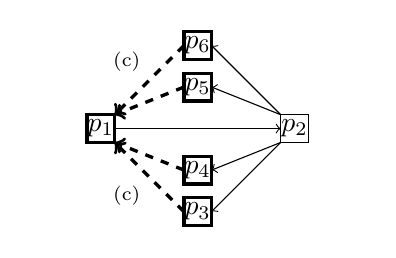
\begin{tikzpicture}[scale=1]

  \newcommand\X{35pt};
  \newcommand\Y{15pt};

  \draw(-0.75*\X, 0pt); %% positioning
  \draw( 2.75*\X, 0pt); %% positioning

  \scriptsize
  \draw[->](5+0*\X, 0*\Y) -- (-5+ 2*\X, 0*\Y);
  \draw[->] (-5+2*\X, 5pt) -- (5+\X, \Y);
  \draw[->] (-5+2*\X, 5pt) -- (5+\X, 2*\Y);
  \draw[->] (-5+2*\X, -5pt) -- (5+\X, -\Y);
  \draw[->] (-5+2*\X, -5pt) -- (5+\X, -2*\Y);

  \draw[->,dashed, very thick](-5+\X, 2*\Y) --
  node[anchor=south east]{(c)} ( 5pt,5pt);
  \draw[->,dashed, very thick](-5+\X, 1*\Y) -- ( 5pt,5pt);
  \draw[->,dashed, very thick](-5+\X, -1*\Y) -- ( 5pt,-5pt);
  \draw[->,dashed, very thick](-5+\X, -2*\Y) --
  node[anchor=north east]{(c)}( 5pt,-5pt);

  \normalsize
  \draw[fill=white, very thick]
  (0*\X, 0*\Y) node{$p_1$} +(-5pt,-5pt) rectangle +(5pt,5pt);
  \draw[fill=white]
  (2*\X, 0*\Y) node{$p_2$} +(-5pt,-5pt) rectangle +(5pt,5pt);

  \draw[fill=white, very thick]
  (1*\X,2*\Y) node{$p_6$} +(-5pt,-5pt) rectangle +(5pt,5pt);
  \draw[fill=white, very thick]
  (1*\X,1*\Y) node{$p_5$} +(-5pt,-5pt) rectangle +(5pt,5pt);
  \draw[fill=white, very thick]
  (1*\X,-1*\Y) node{$p_4$} +(-5pt,-5pt) rectangle +(5pt,5pt);
  \draw[fill=white, very thick]
  (1*\X,-2*\Y) node{$p_3$} +(-5pt,-5pt) rectangle +(5pt,5pt);
 

\end{tikzpicture}}
  \caption{\label{fig:joiningexample}Example of the \SPRAY's joining
    protocol.}
\end{figure*}

\begin{algorithm}

\small
\algrenewcommand{\algorithmiccomment}[1]{\hskip2em$\rhd$ #1}

\newcommand{\comment}[1]{$\rhd$ #1}


\algblockdefx[initially]{initially}{endInitially}
  [0] {\textbf{INITIALLY:}} 

\algblockdefx[pas]{pas}{endPas}
  [0] {\textbf{EVENTS:}}

\newcommand{\LINEFOR}[2]{%
  \algorithmicfor\ {#1}\ \algorithmicdo\ {#2} %
  }

\newcommand{\LINEIFTHEN}[2]{%
  \algorithmicif\ {#1}\ \algorithmicthen\ {#2} %
  }

\newcommand{\INDSTATE}[1][1]{\State\hspace{\algorithmicindent}}

\begin{algorithmic}[1]
  \Statex
  \initially
    \State $\mathcal{P} \leftarrow \varnothing$;
    \hfill \comment{the partial view is a multiset}
    \State $p$ ; \hfill \comment{identity of the local peer}
  \endInitially
  
  \pas
  \Function{onSubs}{$o$} \hfill \comment{$o: origin$}
    \State \LINEFOR{\textbf{each} $\langle q,\,\_\, \rangle \in\mathcal{P}$}
    {$sendTo(q,\, 'fwdSubs',\, o)$;} \label{line:multicast}
    \EndFunction
    \Statex
    \Function{onFwdSubs}{$o$} \hfill \comment{$o: origin$}
    \State $\mathcal{P} \leftarrow
    \mathcal{P}\uplus \left\{\langle o,\, 0 \rangle\right\}$;
    \EndFunction
  \endPas
  
\end{algorithmic}

\caption{\label{algo:joining}The joining protocol of \SPRAY.}
\end{algorithm}

La vue partielle est un multiensemble de couples $\langle n,\, age\rangle$ qui
associe à chaque voisin $n$ l'âge $age$. Ce multiensemble permet de gérer les
doublons. L'âge joue le même rôle que dans \CYCLON, çàd qu'il accélère la
suppression des pairs qui sont sortis ou ont crash. L'évenement $onSubs$ est
appelé chaque fois qu'un pair rejoins le réseau via ce contact. $onSubs$
redirige l'identité du pairs à tous ses voisins, indépendament de
l'âge. L'évenement $onFwdSubs$ est déclanché lorsqu'un pair reçoit une telle
identité redirigée. $onFwdSubs$ ajoute la référence en initialisant son âge à
$0$.

La figure~\ref{fig:joiningexample} décrit un scenario où le pair $p_1$ contacte
le pair $p_2$ afin de rejoindre le réseau composé de $\{p_2$, $p_2$, $p_4$,
$p_5$, $p_6\}$. Pour simplifier, la figure ne montre que les arcs nouvellement
introduit ainsi que le voisinage de $p_1$ et $p_2$. Le pair $p_1$ ajoute
directement $p_2$ dans sa vue partielle. Ce dernier redirige l'identité de $p_1$
à chacun de ses voisins.  Chacun de ces voisins ajoute alors $p_1$ à leur vue
partielle. Au total, \SPRAY établie 5 connexions. Le réseau en résultant est
connecté.

Malheureusement, les vues partiels des derniers arrivant sont clairement
déséquilibrés comparé au reste du réseau. De ce fait, ils violent la première
condition de l'énoncé du problème (REF). Le processus de mélange décrit dans la
prochaine section a pour but de ré-équilibrer les vues partielles.

\subsection{Échanger son voisinage}

Au contraire de \CYCLON, \SPRAY mélange des vues partielles dont les tailles
peuvent être différentes. Ce processus à pour but d'équilibrer les tailles de
vue partielles ainsi que de mélanger les références à l'interieur de celles-ci.
Ce processus à pour contrainte de conserver l'exact même nombre d'arcs.

Les deux pairs impliqués dans le mélange s'envoient l'un l'autre la moitié de
leur vue partielle. Après l'intégration de ces nouvelles références, la taille
de leur vue partielle tend vers la moyenne, et la somme globale en demeure
inchangée. Dans ce but, les vues partielles sont des multiensembles. Ainsi, si
un pair réçoit une référence déjà connue, il la conserve en tant que doublon.
De cette façon, le nombre d'arcs reste constant.

Si les doublons ont un impact négatif sur les propriétés du réseau, la plupart
de ceux-ci disparaissent après le processus de mélange. En proportion, ils
deviennent négligeable dès lors que le réseau grandit.

\begin{algorithm}[h]
  
\small
\algrenewcommand{\algorithmiccomment}[1]{\hskip2em$\rhd$ #1}

\newcommand{\comment}[1]{$\rhd$ #1}

\algblockdefx[act]{act}{endAct}
  [0] {\textbf{ACTIVE THREAD:}}

\algblockdefx[pas]{pas}{endPas}
  [0] {\textbf{PASSIVE THREAD:}}


\newcommand{\LINEFOR}[2]{%
  \algorithmicfor\ {#1}\ \algorithmicdo\ {#2} %
  }

\newcommand{\LINEIFTHEN}[2]{%
  \algorithmicif\ {#1}\ \algorithmicthen\ {#2} %
  }

\newcommand{\INDSTATE}[1][1]{\State\hspace{\algorithmicindent}}

\begin{algorithmic}[1]
  \Statex
  \act
    \Function{loop}{ } \hfill \comment{Every $\Delta\,t$}
    \State $\mathcal{P} \leftarrow incrementAge(\mathcal{P})$;
    \State \textbf{let} $ \langle q,\, age \rangle \leftarrow getOldest(\mathcal{P})$;
    \State \textbf{let} $sample \leftarrow $ \label{line:samplesize}
    $getSample(\mathcal{P}\setminus\left\{\langle q, age\rangle\right\}, \left \lceil{|\mathcal{P}|\over{2}} \right \rceil-1) \uplus \left\{\langle p, 0 \rangle\right\}$;
    \State $sample \leftarrow replace(sample,\,q,\,p)$; \label{line:replace1}
    \State $sendTo(q,\, 'exchange',\, sample)$;
    \State \textbf{let} $sample'\leftarrow receiveFrom(q)$;
    \State $sample \leftarrow replace(sample,\,p,\,q)$;
    \State $\mathcal{P} \leftarrow (\mathcal{P} \setminus sample) \uplus
    sample'$;
    \EndFunction
  \endAct
  
  \pas
    \Function{onExchange}{$o,\, sample$} \hfill \comment{$o: origin$}
    \State \textbf{let} $sample' \leftarrow getSample(\mathcal{P} ,\, \left\lceil |\mathcal{P}|\over{2} \right\rceil )$;
    \State $sample' \leftarrow replace(sample',\,o,\,p);$ \label{line:replace2}
    \State $sendTo(o ,\, sample')$;
    \State $sample' \leftarrow replace(sample',\,p,\,o)$;
    \State $\mathcal{P} \leftarrow (\mathcal{P} \setminus sample') \uplus
    sample$; 
    \EndFunction
  \endPas
  
\end{algorithmic}

  \caption{\label{algo:scamplon}The cyclic protocol of \SPRAY.}
\end{algorithm}

L'algorithme~\ref{algo:scamplon} montre la partie periodic de \SPRAY éxécutée
par chaque pair. Il est divisé en deux parties, à savoir le processus actif qui
est appelé régulièrement afin d'initier un mélange de vues, et le processus
passif qui réagit au message du processus actif. Les fonctions qui ne sont pas
explicitement définies sont les suivantes:
\begin{compactitem}
\item $incrementAge(view)$ : incrémente l'âge des éléments présent dans la vue
  $view$ et retourne la vue modifiée.
\item $getOldest(view)$ : retourne le plus vieu des pairs présent dans la vue.
\item $getSample(view,\, size)$ : retourne un échantillon de la vue contenant $size$
  éléments.
\item $replace(view,\,old,\,new)$ : remplace les occurrences de $old$ par $new$ dans
  la vue $view$.
\item $rand()$ : retourne un nombre flottant aléatoire entre $0$ et $1$.
\end{compactitem}

Dans le processus actif, la fonction $loop$ est appelée tous les intervals
$\Delta$ de temps. Tout d'abord, la fonction incrémente l'age de chacun des
voisins dans la vue partielle $\mathcal{P}$. Ensuite, le pair le plus âgé $q$
est choisit afin d'initier un échange. Si le pair $q$ ne peut être joint (car il
est parti ou a crash), alors le pair $p$ éxecute la fonction qui gère ce cas
(voir la section suivante). Ceci est répété jusqu'à ce que $p$ trouve un pair
avec qui communiquer. Ainsi, le vieillissement comme héritage de \CYCLON permet
d'accélérer la suppression des références invalides. Une fois que le pair
initiateur $p$ a trouvé un pair avec qui effectuer l'échange, il selectionne un
échantillon de sa vue partielle tout en excluant la référence à $q$ et en
s'incluant lui-même. La taille de l'échantillon correspond à la moitié de la
taille de la vue partielle avec au minimum $1$ pair : sa propre référence
(cf. Line~\ref{line:samplesize}). La réponse de $q$ contient également la moitié
de sa vue partielle. Puisque les pairs ne peuvent apparaitre plusieurs fois dans
$\mathcal{P}$, les pairs impliqués dans le processus d'échange peuvent envoyer
des références cet autre pair ($p$ envoie des références $q$ à $q$). Sans
procédures supplémentaires, ce genre de comportement peut créer des boucles
locales ($q$ a $q$ dans sa vue partielle) ce qui est hautement indésirable. Les
lignes~\ref{line:replace1},~\ref{line:replace2} permettent de remplacer les
auto-références dans l'échantillon. Enfin, chez les deux pairs, l'échantillon envoyé 
est supprimé de la vue partielle, et l'échantillon réçu est ajouté.

La figure~\ref{fig:cyclicexample} décrit le méchanisme périodique de \SPRAY. Ce
scénario suit celui de la figure~\ref{fig:joiningexample}: le pair $p_1$ vient
de rejoindre le réseau. Le pair $p_6$ initie un échange avec $p_1$ (qui est ici
le plus vieux dans sa vue partielle). $p_6$ choisit
$\left\lceil{|\mathcal{P}_6|\div 2}\right\rceil = 1$ aléatoirement parmis son
voisinnage. Dans ce cas, il choisit $p_9$ parmis $\{p_9,\,p_8,\,p_7\}$. Il
envoie à $p_1$ cet échantillon auquel est ajoutée sa propre identité. En
réponse, le pair $p_1$ choisit
$\left\lceil{|\mathcal{P}_1|\div 2}\right\rceil = 1$ pair de sa vue
partielle. L'échantillon composé du seul voisin $p_2$ est envoyé. Immédiatement
après, $p_1$ peut supprimer l'échantillon envoyé et intégrer celui réçu
résultant en une vue partielle composée de $\{p_6,\, p_9\}$. De la même façon,
après réception de l'échantillon de $p_1$, $p_6$ supprime et intègre les
échantillons adéquats, résultant en une vue partielle composée de
$\{p_2,\,p_7,\,p_8\}$.

La procédure d'échange tend à réduire l'écart de taille des vues partielles. De
plus, elle disperse les références aux pairs afin de supprimer les groupes trop
denses dûes à la procédure d'entrée dans le réseau.

En ce qui concerne le temps de converge de l'algorithme de mélange, il existe
une relation proche entre \SPRAY et le protocole d'aggrégation proactive
présenté dans~\cite{jelasity2004epidemic, montresor2004robust}. Celui-ci déclare
que, sous l'hypothèse d'un échantillonnage suffisamment aléatoire, la valeur
moyenne $\mu$ et la variance $\sigma^2$ a un cycle $i$ sont :
\begin{center}
  $\mu_i = {1\over{|\mathcal{N}|}} \sum\limits_{x \in \mathcal{N}} a_{i,\,x}$
  \hfill
  $\sigma^2_i = {1\over{|\mathcal{N}|-1}}\sum\limits_{x \in \mathcal{N}}
  (a_{i,\,x} - \mu_i)^2$
\end{center}
avec $a_{i,\,x}$ la valeur stockée par le pair $p_x$ au cycle $i$. La variance
estimée doit converger en 0 au cours des cycles. En d'autres termes, les valeurs
se rapprochent les unes des autres au cours des cycles. Dans le cas de \SPRAY,
cette valeur $a_{i,\,x}$ est la taille de la vue partiel du pair $p_x$ au cycle
$i$. En effet, chaque échange du pair $p_1$ et du pair $p_2$ est une aggrégation
dont le résultat est :
$|\mathcal{P}_1|\approx|\mathcal{P}_2|\approx{(|\mathcal{P}_1| +
  |\mathcal{P}_2|) \div 2}$.
De plus, à chaque cycle, chaque pair est impliqué dans un protocole d'échange au
moins une fois (celui qu'ils initient), and, dans le meilleur des cas
$1+Poisson(1)$ (celui qu'ils initient et, en moyenne, celui qu'ils réçoivent
d'un autre pair). Cette relation étant établie, nous en déduisons que la taille
des vues partielles des pairs de \SPRAY converge en temps exponentiel vers la
moyenne globale. De plus, chaque cycle réduit la variance du système global à un
taux compris entre ${1\div 2}$ et $1\div ({2\sqrt{\text{e}}})$.

\subsection{Quitter le réseau}

Avec \SPRAY, les pairs peuvent quitter le réseau sans alerter qui que ce
soit. Nous ne faisons pas de distinctions particulières entre les départs et les
crashs. Toutefois, le protocole doit réagir à ces deux cas. En effet, sans
réactions, le réseau pourrait s'éffondrer pour cause de suppression d'arcs trop
zélé. Lorsqu'un pair rejoint le réseau, il y injecte $1+\ln(|\mathcal{N}|)$
arcs. Néanmoins, après plusieurs échanges, la vue partielle du pair rejoignant
le réseau est remplie par d'autres références. Ainsi, quand il quitte le réseau,
il entraine la suppression de $\ln(|\mathcal{N}|)$ arcs de sa vue partielle, et
$\ln(|\mathcal{N}|)$ arcs des pairs l'ayant dans leur vue partielle. Par
conséquent, sans moyens de gérer les départs, $2\ln(\mathcal{N}|)$ arcs sont
supprimés au lieu des $1+\ln(|\mathcal{N}|)$. Afin d'y remedier, chaque pair qui
détecte un crash peut rétablir une connexion avec l'un de ces voisins en
introduisant un doublon (doublon qui disparaitra rapidement après quelques
protocoles d'échange). La probabilité de réétablir une connexion est
$1-1\div{|\mathcal{P}|}$. Puisque ${|\mathcal{P}|}\approx \ln(|\mathcal{N}|)$
pairs ont detecté le crash dans leur vue partielle, il est probable qu'ils
recréent tous la connexion perdue, à l'exception d'un pair. De ce fait,
lorsqu'un pair quitte le réseau, il entraine la suppression d'un nombre d'arcs
correspondant approximativement au nombre d'arcs ajouté lors de la dernière
entrée de pair.

\begin{algorithm}[h]
  
\small
\algrenewcommand{\algorithmiccomment}[1]{\hskip2em$\rhd$ #1}

\newcommand{\comment}[1]{$\rhd$ #1}

\newcommand{\LINEFOR}[2]{%
  \algorithmicfor\ {#1}\ \algorithmicdo\ {#2} %
  }

\newcommand{\LINEIFTHEN}[2]{%
  \algorithmicif\ {#1}\ \algorithmicthen\ {#2} %
  }

\newcommand{\INDSTATE}[1][1]{\State\hspace{\algorithmicindent}}

\begin{algorithmic}[1]
  \Function{onPeerDown}{$q$} \hfill \comment{$q$: crashed/departed peer}  
  \State \textbf{let} $occ \leftarrow 0$;

  \For{\textbf{each} $\langle n,\,age\rangle \in \mathcal{P}$}
  \hfill \comment{remove and count}
  \If {($n=q$)}
  \State $\mathcal{P} \leftarrow \mathcal{P}\setminus \{\langle n,\,age\rangle \}$;
  \State $occ \leftarrow occ + 1$;
  \EndIf
  \EndFor

  \For{$i\leftarrow 0$ \textbf{to} $occ$} 
  \hfill \comment{probabilistically duplicates}
  \If{($rand()>{1\over{|\mathcal{P}|+occ}}$)}
  \State \textbf{let} $\langle n,\,\_ \,\rangle \leftarrow
  \mathcal{P}[\left\lfloor rand()*|\mathcal{P}|\right\rfloor]$;
  \State $\mathcal{P} \leftarrow \mathcal{P} \uplus
  \left\{\langle n,\, 0\rangle\right\}$;
  \EndIf
  \EndFor
  
  \EndFunction
  \Statex
  \Function{onArcDown}{$q,\,age$}
  \hfill \comment{$q$: arrival of the arc down}  
  \State $\mathcal{P} \leftarrow \mathcal{P}\setminus \{\langle q,\,age\rangle \}$;
  \State \textbf{let} $\langle n,\,\_ \,\rangle \leftarrow
  \mathcal{P}[\left\lfloor rand()*|\mathcal{P}|\right\rfloor]$;
  \State $\mathcal{P} \leftarrow \mathcal{P} \uplus
  \left\{\langle n,\, 0\rangle\right\}$;
  \hfill \comment{systematically duplicates}
  \EndFunction

\end{algorithmic}

  \caption{\label{algo:unreachable}The crash/departure handler of \SPRAY.}
\end{algorithm}

L'algorithme~\ref{algo:unreachable} montre la manière selon laquelle \SPRAY gère
les départs et crashs. La fonction $onPeerDown$ montre la réaction de \SPRAY
lorsque le pair $q$ est detecté comme parti ou défaillant. Dans un premier
temps, la fonction compte les occurences du pair $q$ dans la vue partielle et
les supprimes. Dans un second temps, une boucle ajoute de manière probabiliste
des doublons de références à des pairs déjà connus. La probabilité dépend de la
taille de la vue partielle avant la suppression.

\begin{figure*}
  \centering
  \subfloat[Figure A][Peer $p_1$ crashes.]{
    
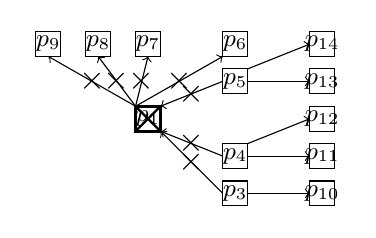
\begin{tikzpicture}[scale=0.9]

  \newcommand\X{35pt};
  \newcommand\Y{15pt};
  \large
  \draw[->](-5+\X, 1*\Y) --node{$\times$} ( 5pt,5pt);
  \draw[->](-5+\X, -1*\Y) --node{$\times$} ( 5pt,-5pt);
  \draw[->](-5+\X, -2*\Y) --node{$\times$} ( 5pt,-5pt);

  \draw[->](-5pt,5pt)--node{$\times$}(-10-2*\Y,-5+2*\Y); %% 1 -> 9
  \draw[->](-5pt,5pt)--node{$\times$}(-5-1*\Y,-5+2*\Y); %% 1 ->8 
  \draw[->](-5pt,5pt)--node{$\times$}(0pt,-5+2*\Y); %% 1 -> 7
  \draw[->](-5pt,5pt)--node{$\times$}(-5+\X,-5+2*\Y); %% 1 -> 6
  \normalsize
  \draw[->](5+ 1*\X, 5+ 1*\Y)--(-5+2*\X, 2*\Y); %% 5 -> 14
  \draw[->](5+1*\X,  1*\Y)--(-5+2*\X, 1*\Y); %% 5 -> 13 
  
  \draw[->](5+\X, 5-\Y) -- (-5+2*\X,0pt); %% 4 -> 12
  \draw[->](5+\X, -\Y) -- (-5+2*\X, -\Y); %% 4 -> 11
  
  \draw[->](5+\X, -2*\Y) -- (-5+2*\X, -2*\Y);
  
  \small
  \draw[fill=white,very thick]
  (0*\X, 0*\Y) node{$p_1$} +(-5pt,-5pt) rectangle +(5pt,5pt);
  \draw[thick] (-5pt,-5pt) -- (5pt,5pt);
  \draw[thick] (-5pt, 5pt) -- (5pt,-5pt);
  
  \draw[fill=white]
  (1*\X,1*\Y) node{$p_5$} +(-5pt,-5pt) rectangle +(5pt,5pt);
  \draw[fill=white]
  (1*\X,-1*\Y) node{$p_4$} +(-5pt,-5pt) rectangle +(5pt,5pt);
  \draw[fill=white]
  (1*\X,-2*\Y) node{$p_3$} +(-5pt,-5pt) rectangle +(5pt,5pt);

  \draw[fill=white](\X,2*\Y) node{$p_6$} +(-5pt,-5pt) rectangle +(5pt,5pt);

  \draw[fill=white]( 0*\X,2*\Y)
  node{$p_7$} +(-5pt,-5pt) rectangle +(5pt,5pt);
  \draw[fill=white](-5+-\Y,2*\Y)node{$p_8$} +(-5pt,-5pt) rectangle +(5pt,5pt);
  \draw[fill=white](-10+-2*\Y,2*\Y) node{$p_9$} +(-5pt,-5pt) rectangle +(5pt,5pt);
  
  \draw[fill=white](2*\X,2*\Y)node{$p_{14}$} +(-5pt,-5pt) rectangle +(5pt,5pt);
  \draw[fill=white](2*\X,1*\Y)node{$p_{13}$} +(-5pt,-5pt) rectangle +(5pt,5pt);
  \draw[fill=white](2*\X,0*\Y)node{$p_{12}$} +(-5pt,-5pt) rectangle +(5pt,5pt);
  \draw[fill=white](2*\X,-1*\Y)node{$p_{11}$}+(-5pt,-5pt) rectangle +(5pt,5pt);
  \draw[fill=white](2*\X,-2*\Y)node{$p_{10}$}+(-5pt,-5pt) rectangle +(5pt,5pt);

\end{tikzpicture}}
  \hspace{10pt}
  \subfloat[Figure B][The peers $p_{3-5}$ notice that they cannot
  reach $p_1$ anymore.]{
    
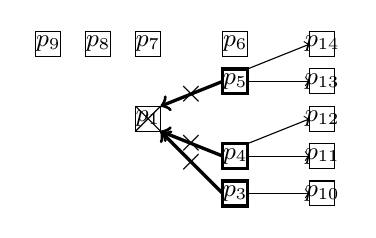
\begin{tikzpicture}[scale=0.9]

  \newcommand\X{35pt};
  \newcommand\Y{15pt};

  \large
  \draw[->, very thick](-5+\X, 1*\Y) -- node{$\times$} ( 5pt,5pt);
  \draw[->, very thick](-5+\X, -1*\Y) --node{$\times$} ( 5pt,-5pt);
  \draw[->, very thick](-5+\X, -2*\Y) --node{$\times$} ( 5pt,-5pt);

  \normalsize

  \draw[->](5+ 1*\X, 5+ 1*\Y)--(-5+2*\X, 2*\Y); %% 5 -> 14
  \draw[->](  5+1*\X, 1*\Y)--(-5+2*\X, 1*\Y); %% 5 -> 13 (v)
  
  \draw[->](5+\X, 5-\Y) -- (-5+2*\X,0pt); %% 4 -> 12
  \draw[->](5+\X, -\Y) -- (-5+2*\X, -\Y); %% 4 -> 11
  
  \draw[->](5+\X, -2*\Y) -- (-5+2*\X, -2*\Y);
  
  \small
  \draw[fill=white]
  (0*\X, 0*\Y) node{$p_1$} +(-5pt,-5pt) rectangle +(5pt,5pt);
  \draw (-5pt,-5pt) -- (5pt,5pt);
  \draw (-5pt, 5pt) -- (5pt,-5pt);
  
  \draw[fill=white, very thick]
  (1*\X,1*\Y) node{$p_5$} +(-5pt,-5pt) rectangle +(5pt,5pt);
  \draw[fill=white, very thick]
  (1*\X,-1*\Y) node{$p_4$} +(-5pt,-5pt) rectangle +(5pt,5pt);
  \draw[fill=white, very thick]
  (1*\X,-2*\Y) node{$p_3$} +(-5pt,-5pt) rectangle +(5pt,5pt);

  \draw[fill=white](\X,2*\Y) node{$p_6$} +(-5pt,-5pt) rectangle +(5pt,5pt);

  \draw[fill=white]( 0*\X,2*\Y)
  node{$p_7$} +(-5pt,-5pt) rectangle +(5pt,5pt);
  \draw[fill=white](-5+-\Y,2*\Y)node{$p_8$} +(-5pt,-5pt) rectangle +(5pt,5pt);
  \draw[fill=white](-10+-2*\Y,2*\Y) node{$p_9$} +(-5pt,-5pt) rectangle +(5pt,5pt);
  
  \draw[fill=white](2*\X,2*\Y)node{$p_{14}$} +(-5pt,-5pt) rectangle +(5pt,5pt);
  \draw[fill=white](2*\X,1*\Y)node{$p_{13}$} +(-5pt,-5pt) rectangle +(5pt,5pt);
  \draw[fill=white](2*\X,0*\Y)node{$p_{12}$} +(-5pt,-5pt) rectangle +(5pt,5pt);
  \draw[fill=white](2*\X,-1*\Y)node{$p_{11}$}+(-5pt,-5pt) rectangle +(5pt,5pt);
  \draw[fill=white](2*\X,-2*\Y)node{$p_{10}$}+(-5pt,-5pt) rectangle +(5pt,5pt);

\end{tikzpicture}}
  \hspace{10pt}
  \subfloat[Figure C][The peers $p_3$ and $p_5$ choose to establish
  a duplicate with one of their existing neighbor.]{
    
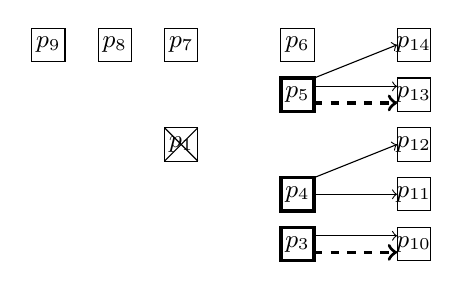
\begin{tikzpicture}[scale=1.2]

  \newcommand\X{35pt};
  \newcommand\Y{15pt};

  \draw[->](5+ 1*\X, 5+ 1*\Y)--(-5+2*\X, 2*\Y); %% 5 -> 14
  \draw[->](5+1*\X, 2.5+ 1*\Y)--(-5+2*\X, 2.5+ 1*\Y); %% 5 -> 13 (^)
  \draw[->,dashed, very thick]
  (  5+1*\X,-2.5+1*\Y)--(-5+2*\X,-2.5+1*\Y); %% 5 -> 13 (v)
  
  \draw[->](5+\X, 5-\Y) -- (-5+2*\X,0pt); %% 4 -> 12
  \draw[->](5+\X, -\Y) -- (-5+2*\X, -\Y); %% 4 -> 11
  
  \draw[->](5+\X, 2.5-2*\Y) -- (-5+2*\X, 2.5-2*\Y);
  \draw[->,dashed, very thick](5+\X, -2.5-2*\Y) -- (-5+2*\X , -2.5-2*\Y);
  
  \small
  \draw[fill=white]
  (0*\X, 0*\Y) node{$p_1$} +(-5pt,-5pt) rectangle +(5pt,5pt);
  \draw (-5pt,-5pt) -- (5pt,5pt);
  \draw (-5pt, 5pt) -- (5pt,-5pt);
  
  \draw[fill=white, very thick]
  (1*\X,1*\Y) node{$p_5$} +(-5pt,-5pt) rectangle +(5pt,5pt);
  \draw[fill=white, very thick]
  (1*\X,-1*\Y) node{$p_4$} +(-5pt,-5pt) rectangle +(5pt,5pt);
  \draw[fill=white, very thick]
  (1*\X,-2*\Y) node{$p_3$} +(-5pt,-5pt) rectangle +(5pt,5pt);

  \draw[fill=white](\X,2*\Y) node{$p_6$} +(-5pt,-5pt) rectangle +(5pt,5pt);

  \draw[fill=white]( 0*\X,2*\Y)
  node{$p_7$} +(-5pt,-5pt) rectangle +(5pt,5pt);
  \draw[fill=white](-5+-\Y,2*\Y)node{$p_8$} +(-5pt,-5pt) rectangle +(5pt,5pt);
  \draw[fill=white](-10+-2*\Y,2*\Y) node{$p_9$} +(-5pt,-5pt) rectangle +(5pt,5pt);
  
  \draw[fill=white](2*\X,2*\Y)node{$p_{14}$} +(-5pt,-5pt) rectangle +(5pt,5pt);
  \draw[fill=white](2*\X,1*\Y)node{$p_{13}$} +(-5pt,-5pt) rectangle +(5pt,5pt);
  \draw[fill=white](2*\X,0*\Y)node{$p_{12}$} +(-5pt,-5pt) rectangle +(5pt,5pt);
  \draw[fill=white](2*\X,-1*\Y)node{$p_{11}$}+(-5pt,-5pt) rectangle +(5pt,5pt);
  \draw[fill=white](2*\X,-2*\Y)node{$p_{10}$}+(-5pt,-5pt) rectangle +(5pt,5pt);

\end{tikzpicture}}
  \caption{\label{fig:crashexample}Example of \SPRAY's crash/leaving
    handler. }
\end{figure*}

La figure~\ref{fig:crashexample} montre le fonctionnement de la gestion des
pairs detecté comme étant parti ou défaillant. Le pair $p_1$ quitte le réseau
sans en informer le réseau. Avec lui, $7$ connexions sont inutilisables. Les
pairs $p_3$, $p_4$, et $p_5$ ont toujours une référence vers $p_1$ dans leur vue
partielle. Le pair $p_5$ a $1-{1\div{|\mathcal{P}_5|}}={2\div{3}}$ chances de
remplacer la connexion. Dans ce cas, il double la référence à $p_{13}$. De la
même manière, $p_3$ et $p_4$ détectent $p_1$ comme étant injoignable et agissent
en conséquence. Seul $p_3$ crée un doublon remplaçant. Au total, $5$ connexions
ont été supprimées.

L'exemple montre que certains des pairs ont rétabli une connexion lorsqu'ils ont
détécté qu'un pair était injoignable. La probabilité dépend de la vue partielle
de chacun de ces pairs. En moyenne, l'un de ces pairs va vraisemblablement
supprimer l'arc inutilisable alors que les autres vont simplement le
remplacer. Dans l'exemple, le pair $p_1$ a injecté $5$ arcs lors de son entrée
dans le réseau. $7-2 = 5$ arcs ont été supprimés lors de son départ. Le nombre
global d'arcs dans le réseau reste d'ordre logarithmique comparé à la taille du
réseau. Toutefois, nous remarquons que la connectivité n'est pas entièrement
garantie (seulement avec la forte probabilité impliquée par les graphes
aléatoires). En effet, si le pair $p_1$ est le seul pont entre deux groupes de
pairs, ajouter des arcs n'est pas suffisant pour garantir la connectivité.

L'algorithme~\ref{algo:unreachable} montre aussi que \SPRAY distingue les pairs
qui sont injoignables des arcs inutilisables. En effet, la fonction $onArcDown$
gère les connexions dont la création a échoué. Ces arcs sont systématiquement
remplacés par un doublon. De ce fait, le nombre d'arc reste bien constant. La
distinction $onPeerDown$ avec $onArcDown$ est necessaire car la première doit
supprimer une petite quantité d'arcs. Sans cette suppression, le nombre d'arcs
augmenterait de manière incontrollée avec les entrées et sorties de pairs.

%%% Local Variables:
%%% mode: latex
%%% TeX-master: "../../paper"
%%% End:
